\documentclass[11pt]{article}
\usepackage[margin=1in]{geometry}
\usepackage{amsmath,amssymb,amsthm}
\usepackage{graphicx,booktabs}
\usepackage[round,authoryear]{natbib}
\usepackage[hidelinks]{hyperref}

\newtheorem{theorem}{Theorem}
\newtheorem{proposition}{Proposition}
\newtheorem{lemma}{Lemma}
\newtheorem{corollary}{Corollary}
\theoremstyle{remark}
\newtheorem{remark}{Remark}

\newcommand{\pr}{\mathrm{pr}}
\newcommand{\LC}{\mathcal{L}}
\newcommand{\E}{E}

\title{Noisy calibration and latent coverage under log-concavity}
\author{Kun woo Park}
\date{}

\begin{document}
\maketitle

\begin{abstract}
Prediction intervals for a latent quantity, such as the true mean of an area that was never sampled, are often calibrated on noisy proxies whose error variances are known. For symmetric unimodal latent errors Anderson's theorem makes such calibration conservative. We ask what can be guaranteed without symmetry. Over all log-concave latent laws, we characterize the smallest latent radius implied by a noisy coverage level, reduce it exactly to a two-parameter family with closed-form Gaussian convolutions, and bound it from above by a branch and bound whose closed forms are evaluated in double precision with a margin. When the noise is small, noisy calibration can undercover the latent target at every coverage level. The radius shortfall is at most $c_q x^{1/2}$ for every noise-to-threshold variance ratio $x$, and this constant is sharp as $x \to 0$. A finite-sample slack of $10^{-3}$ in the calibrated level at $q = 0.9$ removes the shortfall at every noise level, and a slack below $7.9\times10^{-4}$ does not, and above a critical level the noisy threshold may be shrunk. Under heterogeneous independent noise the same Beta quantile still gives a conservative calibration level, by Hoeffding's comparison of Poisson-binomial and binomial tails. The small-noise bound and the slack result need only bi-log-concavity of the latent distribution function. This yields a finite-sample procedure whose conditional reliability holds for every log-concave latent law.
\end{abstract}

\noindent\textit{Some key words}: Conformal prediction; Deconvolution; Localization; Log-concavity; Measurement error; Small area estimation.

\section{Introduction}

Suppose a residual $W$, the latent target minus a centre fitted on independent training data, is observed only through $V = W + e$ with $e \sim N(0, D)$ independent of $W$ and $D$ known. This is the position of a survey statistician who calibrates a prediction interval for the true mean of an unsampled area on the direct estimates of sampled areas \citep{fay1979}, and of a conformal analyst whose calibration responses carry measurement error \citep{einbinder2024, cohen2025}. The threshold $t$ that gives the noisy scores coverage $p$ is observable. The question is what radius gives the latent residual coverage $q$.

If $W$ is symmetric and unimodal, Anderson's theorem \citep{anderson1955} gives $\pr(|W + e| \le t) \le \pr(|W| \le t)$, so the noisy threshold is conservative; \citet{einbinder2024} use this for conformal prediction with noisy labels. Without symmetry only shape-free statements are available. If the noise has median zero, a noisy interval of level $1 - \alpha$ covers the latent value with probability at least $1 - 2\alpha$, and noisy coverage can exceed latent coverage \citep{guille2024}. \citet{cohen2025} estimate the noise-free threshold by deconvolution, but give no finite-sample guarantee. Worst-case coverage over latent laws that are compatible with noisy observations also underlies the robust empirical Bayes intervals of \citet{armstrong2022}, which constrain moments of the latent law and cover sampled units. Conformal intervals under heteroscedastic measurement error cover the noisy response \citep{giertych2024}. Interval methods for small areas likewise target sampled areas \citep{chatterjee2008, yoshimori2014, bersson2024, zhang2026}. We study the problem over the class $\LC$ of log-concave laws on the real line, including point masses. This class is closed under convolution, conditioning on intervals, translation and scaling, and it contains the usual models for regression residuals.

After scaling $t$ to $1$, write $x = D/t^2$, let $Z \sim N(0,1)$, and define
\begin{equation}\label{eq:R}
R_{p,q}(x) = \sup\{ Q_q(|W|) : W \in \LC,\ \pr(|W + x^{1/2}Z| \le 1) \ge p \},
\end{equation}
where $Q_q$ denotes the lower $q$-quantile, and $R_{p,q}(x) = -\infty$ if nothing is feasible, which happens exactly when $\pr(|x^{1/2}Z| \le 1) < p$. If calibration certifies noisy coverage at least $p$ at threshold $t$, then $t\,R_{p,q}(D/t^2)$ is the smallest radius that guarantees latent coverage $q$ for every log-concave latent law. This is sharpness within the class and the single constraint; it is not optimality among all procedures that use the whole calibration sample.

Our results are as follows. The supremum in \eqref{eq:R} may be computed over point masses and log-affine densities on a segment, and for these the constraint has a closed form (\S\ref{sec:reduction}). For every $q$ and every $x$, $R_{q,q}(x) \le 1 + c_q x^{1/2}$ with an explicit $c_q > 0$, and the constant is attained as $x \to 0$. A finite-sample slack $p - q$ of order $10^{-3}$ makes $R_{p,q}(x) \le 1$ for all $x$ (\S\ref{sec:small}). A monotone branch and bound certifies $R_{p,q}$ to a relative accuracy of $3\times 10^{-4}$ over most of its range. With heterogeneous known noise the same Beta quantile remains a conservative level for the average distribution function, by a comparison of \citet{hoeffding1956} and \citet{sen1970}, so the construction gives a finite-sample procedure (\S\ref{sec:procedure}). The small-noise bound and the slack result hold for the larger class of bi-log-concave distribution functions \citep{dumbgen2017}.

\section{Reduction to an extremal family}\label{sec:reduction}

Write $g_x(w) = \pr(|w + x^{1/2}Z| \le 1) = \Phi\{(1-w)/x^{1/2}\} - \Phi\{(-1-w)/x^{1/2}\}$, so that the constraint in \eqref{eq:R} reads $\E\, g_x(W) \ge p$. Let $\mathcal F$ be the family of point masses and of laws with density proportional to $e^{\beta w}$ on a segment $[a,b]$.

\begin{proposition}\label{prop:reduction}
$R_{p,q}(x) = \sup\{Q_q(|W|) : W \in \mathcal F,\ \E\, g_x(W) \ge p\}$. The same holds for any continuous constraint kernel that vanishes at $\pm\infty$, in particular for the average kernel of \S\ref{sec:procedure}.
\end{proposition}

The proof, in the Appendix, conditions $W$ on $[-M, M]$ with $M$ so large that $g_x \le p$ outside. This keeps the constraint at level $p$, because it removes only mass where the kernel is below average. It then applies the localization theorem of \citet{fradelizi2004} to the linear, upper semicontinuous functional $\mu \mapsto -\mu(-s, s)$.

By the symmetry $W \mapsto -W$ we may take $\beta \ge 0$. Integration by parts gives, for $\beta > 0$ and $\sigma = x^{1/2}$,
\begin{equation}\label{eq:closed}
\int_a^b e^{\beta w}\Phi\Big(\frac{c-w}{\sigma}\Big)dw = \frac{1}{\beta}\Big[e^{\beta w}\Phi\Big(\frac{c-w}{\sigma}\Big)\Big]_a^b + \frac{e^{\beta c + \beta^2\sigma^2/2}}{\beta}\Big\{\Phi\Big(\frac{b-c-\beta\sigma^2}{\sigma}\Big) - \Phi\Big(\frac{a-c-\beta\sigma^2}{\sigma}\Big)\Big\},
\end{equation}
so $\pr(W + e \le c)$, and hence the constraint, is a combination of normal distribution functions. Fix the slope and the length and translate $W$ by $c$. Both $c \mapsto \pr(|W + c + e| \le 1)$ and $c \mapsto \pr(|W + c| \le s)$ are log-concave \citep{prekopa1973}. So the feasible translations form an interval, and $Q_q(|W + c|)$ is quasi-convex in $c$ and is maximized at one of the interval's two ends. The supremum in \eqref{eq:R} is therefore a two-dimensional maximization over slope and length of closed-form quantities, each obtained by two root-findings. This computation and an independent differential-evolution search over the three-parameter family agree to $1.5\times10^{-13}$ at all 73 tabulated values of $x \ge 0.006$.

\section{Small noise}\label{sec:small}

The local problem at each endpoint is one-sided. Let
\[
c_{p,q} = \sup\{F_Y^{-1}(q) : Y \in \LC,\ \pr(Y + Z \le 0) \ge p\}, \qquad c_q = c_{q,q}.
\]
Since $W \mapsto (W - t)/D^{1/2}$ preserves $\LC$, the sharp one-sided transfer is exactly $t + D^{1/2}c_{p,q}$ for every $D$. For the exponential tail $Y_{u,b} = b - E$, with $E$ exponential of rate $u$ and independent of $Z$,
\[
\kappa_u(b) = \pr(Y_{u,b} + Z \le 0) = \Phi(-b) + e^{-ub + u^2/2}\,\Phi(b - u),
\]
which is continuous and strictly decreasing in $b$. Let $b_u(p)$ solve $\kappa_u(b) = p$.

\begin{lemma}\label{lem:onesided}
$c_{p,q} = \sup_{u > 0}\{b_u(p) - u^{-1}\log(1/q)\}$. In particular
\[
c_q = \sup_{u>0} u^{-1}\log\{e^{u^2/2}\Phi(b_u - u) + e^{u b_u}\Phi(-b_u)\} > 0, \qquad b_u = b_u(q).
\]
Moreover $q \mapsto c_q$ is nonincreasing.
\end{lemma}

The proof takes a supergradient $u$ of the concave function $\log F_Y$ at the $q$-quantile $v$. Then $F_Y(v + y) \le \min(q e^{uy}, 1)$, which is the distribution function of an exponential tail with the same quantile and a larger constraint value. Monotonicity in $q$ follows by conditioning away left mass. Ball arithmetic gives $c_{0.80} \in [0.0460730, 0.0460731]$, $c_{0.90} \in [0.0190618, 0.0190619]$, $c_{0.95} \in [0.0084075, 0.0084077]$ and $c_{0.99} \in [0.0013950, 0.0013958]$ (Appendix).

\begin{theorem}\label{thm:small}
For every $q \in (0,1)$ and every $x > 0$, $R_{q,q}(x) \le 1 + c_q x^{1/2}$. Moreover $R_{q,q}(x) = 1 + c_q x^{1/2} + o(x^{1/2})$ as $x \to 0$.
\end{theorem}

\begin{proof}[Proof of the upper bound]
Let $W \in \LC$ with $\pr(|W + e| \le 1) \ge q$, and let $\alpha_R = \pr(W + e > 1)$ and $\alpha_L = \pr(W + e < -1)$, so $\alpha_L + \alpha_R \le 1 - q$. The law of $Y = (W - 1)/x^{1/2}$ is log-concave with $\pr(Y + Z \le 0) = 1 - \alpha_R \ge q$. By the definition of $c$ and Lemma~\ref{lem:onesided}, $F_Y^{-1}(1 - \alpha_R) \le c_{1-\alpha_R} \le c_q$, that is, $\pr(W > 1 + c_q x^{1/2}) \le \alpha_R$. The same argument applied to $-W$ gives $\pr(W < -1 - c_q x^{1/2}) \le \alpha_L$. Hence $\pr(|W| \le 1 + c_q x^{1/2}) \ge q$.
\end{proof}

The lower bound places $W = 1 + x^{1/2}Y$ with $Y$ a near-optimal exponential tail, at a level raised by the exponentially small mass that leaks through the far endpoint (Appendix). The extremal laws have a density that rises exponentially towards a cut-off just outside the threshold, with a boundary layer of width $x^{1/2}$. Noise draws more mass inwards across that endpoint than it pushes out, so the effect is of order $x^{1/2}$ rather than the order $x$ that a Taylor expansion suggests. Symmetry removes it entirely.

The argument splits the noisy failure budget between the two endpoints. It extends to $p \ge q$:
\[
R_{p,q}(x) \le 1 + C_{p,q}x^{1/2}, \qquad C_{p,q} = \sup_{\alpha_L+\alpha_R = 1-p}\ \inf_{\beta_L+\beta_R=1-q} \max(c_{1-\alpha_L,1-\beta_L},\, c_{1-\alpha_R,1-\beta_R}),
\]
for every $x$. Numerically the worst split puts the whole budget on one side, so that $C_{p,q} = c_{p,q}$.

\begin{corollary}\label{cor:slack}
If $C_{p,q} \le 0$ then $R_{p,q}(x) \le 1$ for every $x$. If $c_{p,q} > 0$ then $R_{p,q}(x) > 1$ for all small $x$, because the proof of the lower bound in Theorem~\ref{thm:small} gives $R_{p,q}(x) \ge 1 + c_{p,q}x^{1/2} - o(x^{1/2})$ for every $p \ge q$. The smallest slack $p - q$ with $C_{p,q} \le 0$ lies in $(4.3\times10^{-3}, 5.0\times10^{-3}]$, $(7.9\times10^{-4}, 1.0\times10^{-3}]$ and $(1.5\times10^{-4}, 2.0\times10^{-4}]$ at $q = 0.80, 0.90, 0.95$, and so does the smallest slack with $R_{q+\delta,q}(x) \le 1$ for all $x$; double-precision root finding puts it at $4.4\times10^{-3}$, $8.0\times10^{-4}$ and $1.6\times10^{-4}$.
\end{corollary}

For split conformal calibration with $K = 110$ and rank $k = 105$, the order statistic certifies $p_k = 0.9036$ with probability $0.96$. Then $-0.0572 \le C_{0.9036, 0.90} \le -0.057$, so with homogeneous noise the finite-sample procedure never needs widening, and it shrinks the noisy threshold by at least the factor $1 - 0.057x^{1/2}$. The constants $c_{p,q}$ and $C_{p,q}$ are defined for a single Gaussian noise law; for the mixture kernel of \S\ref{sec:procedure} the radius is certified directly.

\begin{corollary}\label{cor:blc}
Let $\mathcal B$ be the class of laws on the real line that are point masses or have a continuous distribution function $F$ with $\log F$ and $\log(1-F)$ concave \citep{dumbgen2017}; $\LC \subset \mathcal B$. Define $R^{\mathcal B}_{p,q}$ by \eqref{eq:R} with $\mathcal B$ in place of $\LC$. Then Lemma~\ref{lem:onesided} holds over $\mathcal B$ with the same $c_{p,q}$, and for $p \ge q$ and every $x > 0$, $R^{\mathcal B}_{p,q}(x) \le 1 + C_{p,q}x^{1/2}$, while $R^{\mathcal B}_{q,q}(x) = 1 + c_qx^{1/2} + o(x^{1/2})$ as $x \to 0$. In particular Corollary~\ref{cor:slack} holds over $\mathcal B$.
\end{corollary}

\begin{proof}
The proof of Lemma~\ref{lem:onesided} uses only the concavity of $\log F_Y$ at the $q$-quantile, so its upper bound holds for every $Y$ with $\log F_Y$ concave; exponential tails are in $\LC$, which gives equality. In the proof of Theorem~\ref{thm:small}, $Y = (W - 1)/x^{1/2}$ has $\log F_Y$ concave, and $(-W - 1)/x^{1/2}$ has a concave log distribution function because $\log(1 - F_W)$ is concave and $F_W$ is continuous. The lower bound uses laws in $\LC \subset \mathcal B$.
\end{proof}

The class $\mathcal B$ allows multimodal densities. Only the small-noise bound and the slack result transfer: the localization of Proposition~\ref{prop:reduction} and the certified values of \S\ref{sec:procedure} use log-concavity of the density. Thus, with homogeneous noise and $p_k - q \ge 10^{-3}$ at $q = 0.9$, the noisy threshold itself covers a bi-log-concave latent residual with probability at least $q$ on the order-statistic event.

Figure~\ref{fig:boundary} shows $R_{q,q}(x) - 1$. Grid maximization, which bounds $R_{q,q}$ from below, puts the critical levels at which $R_{q,q} = 1$ at $x^*(q) \approx 0.034$, $0.017$, $0.0062$ and $0.0012$ for $q = 0.80$, $0.85$, $0.90$ and $0.95$. Below them the noisy threshold must be widened. The largest widening found is $0.37\%$, $0.17\%$, $0.063\%$ and $0.012\%$ respectively; the proved bound is $c_qx^{1/2}$. Above them it may be shrunk, substantially once $x$ exceeds about $0.05$ (Fig.~\ref{fig:certified}).

\begin{figure}[t]
\centering
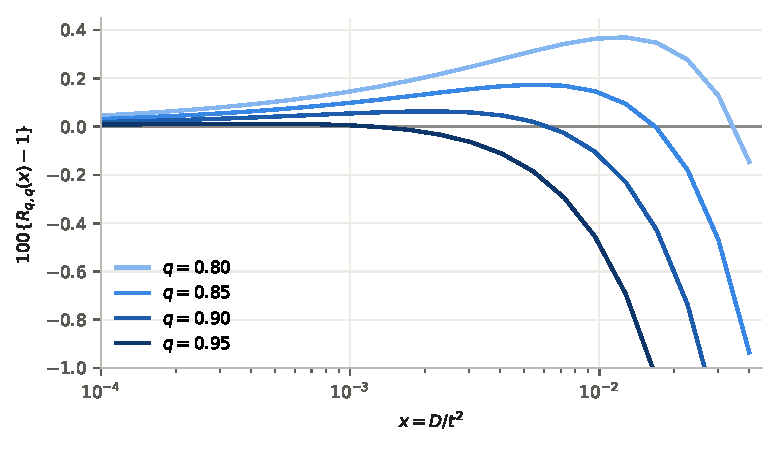
\includegraphics[width=0.75\textwidth]{fig_boundary.pdf}
\caption{Sharp latent radius relative to the noisy threshold, $100\{R_{q,q}(x) - 1\}$, for four coverage levels, computed by grid maximization over the extremal family, which bounds $R_{q,q}$ from below. Above zero the noisy threshold must be widened; below zero it may be shrunk.}
\label{fig:boundary}
\end{figure}

\section{Certified values and a finite-sample procedure}\label{sec:procedure}

\subsection{Certification}

Write a member of $\mathcal F$ with $\beta \ge 0$ as $W = b - Y$, where $Y$ has density proportional to $e^{-\beta y}$ on $[0,\ell]$. The ends of the family are included: $\ell = 0$ or $\beta = \infty$ gives a point mass, and $\ell = \infty$ an exponential tail. $W$ is stochastically increasing in $\beta$ and $b$ and decreasing in $\ell$. On a box of parameters, let $W_{\rm lo}$ and $W_{\rm hi}$ be the stochastically smallest and largest corners. The maps $W \mapsto \pr(W + e \le \pm 1)$ and $W \mapsto \pr(W \le y)$ are expectations of decreasing functions. Hence, for every law in the box,
\begin{align*}
\pr(|W+e| \le 1) &\le \pr(W_{\rm lo} + e \le 1) - \pr(W_{\rm hi} + e \le -1),\\
\pr(|W| \le s) &\ge \pr(W_{\rm hi} \le s) - \pr(W_{\rm lo} \le -s).
\end{align*}
The density bound $\pr(|W+e| \le 1) \le 2\sup f_W$ is also available. A box whose first bound is below $p$, or whose second is at least $q$, contains no law that violates $R_{p,q}(x) \le s$. Branch and bound over boxes then certifies $R_{p,q}(x) \le s$. Here $b$ is confined analytically and $\beta, \ell \in [0,\infty]$ are compactified. Between grid points we use the following result.

\begin{proposition}\label{prop:continuity}
For all $x, h \ge 0$, $R_{p,q}(x + h) \le R_{p,q}(x) + c_q h^{1/2}$.
\end{proposition}

\begin{proof}
If $W$ is feasible at noise level $x + h$, then $W + e_h$, with $e_h \sim N(0,h)$ independent, is log-concave and feasible at level $x$. So $t = Q_q(|W + e_h|) \le R_{p,q}(x)$. Theorem~\ref{thm:small} at scale $t$ then gives $Q_q(|W|) \le t + c_q h^{1/2}$.
\end{proof}

We certified $R_{0.90,0.90}$ and $R_{0.9036,0.90}$ on $x \in [0.002, 0.366]$ with step $5\times 10^{-4}$. The closed forms agree with high-precision quadrature to $10^{-11}$, and boxes are cleared with a margin of $10^{-9}$, so the values are certified up to floating-point evaluation of the closed forms. For $x \in [0.05, 0.3]$ the certified bound exceeds a feasible value by at most a relative $3\times 10^{-4}$. On $[0.02, 0.3]$ it exceeds the earlier uncertified table by at most $0.15\%$. The certificate fails only just before the feasibility edges $x \approx 0.370$ ($p = 0.9$) and $0.361$ ($p = 0.9036$). Below $x = 0.01$ the lookup also uses Theorem~\ref{thm:small} and its $p \ge q$ form, which are within $0.3\%$ of a feasible value there and sharper than the box bounds at $p = 0.9$ (Fig.~\ref{fig:certified}).

\begin{figure}[t]
\centering
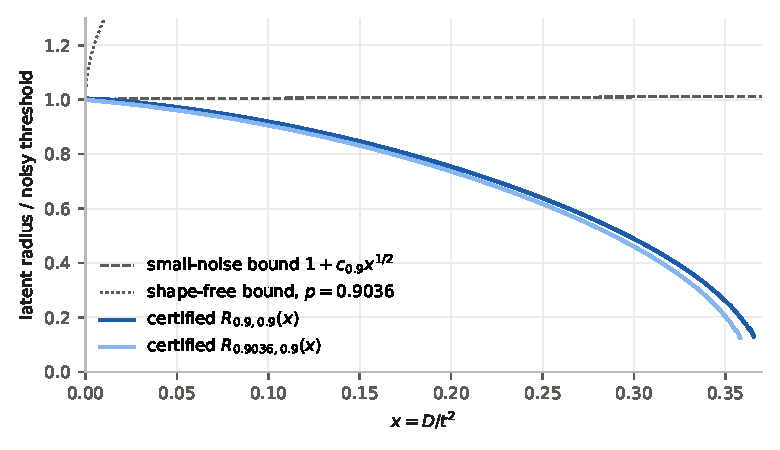
\includegraphics[width=0.75\textwidth]{fig_certified.pdf}
\caption{Certified sharp radius $R_{p,0.9}(x)$ for $p = 0.9$ and for the order-statistic level $p = 0.9036$, with the small-noise bound of Theorem~\ref{thm:small} and the shape-free bound $1 + x^{1/2}z_{1-(p-q)/2}$, which follows from $|W| \le |V| + |e|$.}
\label{fig:certified}
\end{figure}

\subsection{Heterogeneous noise}

Let $W_1, \ldots, W_K, W_{\rm new}$ be independent with law $G \in \LC$, independent of $e_i \sim N(0, D_i)$, with the $D_i$ fixed and known. The calibration scores $V_i = W_i + e_i$ are then independent but not identically distributed. The following is a case of the comparison of \citet{sen1970} between order statistics of heterogeneous laws and those of their average; we give the short proof.

\begin{proposition}\label{prop:beta}
Let $T = |V|_{(k)}$, let $\bar F$ be the average distribution function of the $|V_i|$, assumed continuous, and let $p_k$ be the $\delta$-quantile of the Beta$(k, K+1-k)$ distribution. If $k \ge Kp_k + 1$ then $\pr\{\bar F(T) \ge p_k\} \ge 1 - \delta$.
\end{proposition}

\begin{proof}
$\bar F(T) < p_k$ exactly when $N = \#\{i : |V_i| < \bar F^{-1}(p_k)\} \ge k$. $N$ is a sum of independent indicators with mean $Kp_k$, and $k - 1 \ge Kp_k$. By \citet{hoeffding1956}, $\pr(N \le k-1)$ is minimized when all success probabilities are equal. Hence $\pr(N \ge k) \le \pr\{{\rm Bin}(K, p_k) \ge k\} = \pr\{{\rm Beta}(k, K+1-k) \le p_k\} = \delta$.
\end{proof}

On the event of Proposition~\ref{prop:beta}, the law $G$ satisfies the single linear constraint $\int \bar g\, dG \ge p_k$, with the average kernel $\bar g(w) = K^{-1}\sum_i \pr(|w + e_i| \le T)$. Proposition~\ref{prop:reduction} applies, the box bounds hold term by term, and the heterogeneous rule is
\[
s = T\, R^{\rm mix}_{p_k - \varepsilon,\, q}(D_1/T^2, \ldots, D_K/T^2).
\]
Here $\varepsilon$ bounds, for each data set, the sup-norm error of the average kernel after compressing the $D_i$ to 32 support points: the maximum over a grid of spacing $h = 10^{-3}$ plus $Mh^2/8$, with $M$ a bound on the second derivative; it was about $2\times10^{-4}$. The radius $R^{\rm mix}$ is certified for each data set, and the shape-free bound is used if the certificate fails. Replacing the average kernel by the kernel of a single variance is not safe in general. The mean-variance plug-in is $1.4\%$ too short at $\bar x = 0.2$ with lognormal spread $1$. The minimum-variance plug-in was up to $14\%$ too long in that comparison, but it is not conservative either. Take $W = b - E$ with $E$ exponential of rate $2$ and $b = 1.0435647$, and let the noise be an equal mixture of $N(0, 10^{-8})$ and $N(0, 5\times10^{-4})$. Then the noisy coverage of $[-1, 1]$ exceeds $0.9$, while the radius $1 + c_{0.9}10^{-4}$ given by the smaller variance covers $W$ with probability $0.89977$; this was checked in 192-bit ball arithmetic.

\section{Numerical illustration}\label{sec:numerical}

The target is $\pr_{\mathcal D}\{\pr(W_{\rm new} \in C \mid \mathcal D) \ge 0.90\} \ge 0.95$, with $K = 110$ calibration areas, $\mathrm{var}(W) = 1$ and heterogeneous known noise variances $D_i = 0.577\,L_i/E(L_i)$, $L_i$ lognormal with log-scale $0.7$. Conditional coverage is computed exactly from closed-form latent distribution functions, with 150 replications per law, so the Monte Carlo standard error of a reliability is about $0.018$; for instance $145/150 = 0.967$ has the 95\% binomial interval $[0.924, 0.989]$. The guarantee comes from the theory; the simulation shows widths and failure patterns. Table~\ref{tab:synth} compares four rules:
\begin{itemize}
\item the Fay--Herriot tolerance interval with a parametric bootstrap;
\item noisy split conformal at rank $105$;
\item the log-concave rule with the mean variance plugged into the certified $R_{0.9068,0.9}$, which has no guarantee under heterogeneous noise;
\item the certified heterogeneous rule.
\end{itemize}

\begin{table}[t]
\centering
\caption{Reliability $\pr_{\mathcal D}\{\pr(W_{\rm new}\in C\mid\mathcal D)\ge 0.9\}$ with mean width in parentheses; target reliability $0.95$}
\label{tab:synth}
\begin{tabular}{lcccc}
\toprule
latent law & Fay--Herriot & noisy conformal & log-concave, mean $D$ & heterogeneous \\
\midrule
normal & 0.960 (3.93) & 1.000 (4.96) & 0.980 (4.46) & 0.980 (4.45) \\
Laplace & 0.927 (3.96) & 1.000 (5.15) & 0.987 (4.68) & 0.987 (4.66) \\
centred gamma(2) & 1.000 (3.95) & 1.000 (4.97) & 1.000 (4.46) & 1.000 (4.45) \\
truncated Laplace & 0.847 (3.89) & 1.000 (4.93) & 0.973 (4.43) & 0.967 (4.42) \\
\bottomrule
\end{tabular}
\end{table}

Every heterogeneous radius was certified, at relative tolerance $10^{-3}$ in 368 of 600 data sets, $3\times10^{-3}$ in 222 and $10^{-2}$ in 10, so the shape-free fallback was never used. Certification costs $0.2\%$ of width against the uncertified grid value. Both log-concave rules use the order-statistic level $p_k = 0.9068$ of $\delta = 0.05$. The certified heterogeneous rule meets the target for all four laws. It is only $0.3\%$ shorter than the mean-variance plug-in, so the exact kernel buys validity rather than width here. The order-statistic level accounts for most of the gain over the $p = q$ table: $3.0\%$ of width, of which $1.2\%$ comes from raising $p$ from $0.9036$ to $0.9068$. The heterogeneous rule is $9.5$--$10.5\%$ shorter than noisy conformal. It is $12.5$--$18\%$ longer than the Fay--Herriot tolerance interval, which misses the target under the truncated Laplace law ($0.847$) and falls short under the Laplace law by about $1.3$ standard errors ($0.927$).

In the finite population \texttt{apipop} \citep{lumley2004}, 110 of 325 school districts are used for training and 110 for calibration, with 2 or 3 schools sampled per district. Coverage is the share of the remaining 105 districts that are covered. Design variances are estimated with 1--2 degrees of freedom and plugged in as known by every rule, a case that no guarantee covers.
\begin{itemize}
\item Reliability over four conditions of 120 replications: the heterogeneous rule $0.942$--$0.992$, the mean-variance rule $0.983$--$1.000$, Fay--Herriot $0.908$--$0.992$ (below target in two conditions).
\item The heterogeneous rule at level $p_k$ is $0.8$--$5.2\%$ shorter than the mean-variance rule with the $p = q$ table, mostly because of the level, and $10$--$16\%$ longer than Fay--Herriot.
\end{itemize}

\section{Discussion}

The guarantee is conditional on the calibration sample and concerns a new area whose residual is drawn from the same law $G$ as the calibration residuals, independently. It is not a guarantee for each fixed area, nor a design-based guarantee for a fixed finite population. It assumes that the latent residual is log-concave (bi-log-concave for \S\ref{sec:small}) and that the noise is Gaussian, independent of the latent residual, with fixed and known variances. The latent law is identified from the noisy scores when the Gaussian kernel is known, but a shape constraint cannot be confirmed from a finite sample. Log-concavity is much weaker than the normality used by Fay--Herriot intervals, which missed the target under a truncated Laplace law. Estimated variances require an outer confidence set $\mathcal D_\eta$ for the variances, with radius $T\sup_{d \in \mathcal D_\eta}R^{\rm mix}_{p_k,q}(d/T^2)$ and reliability $1 - \delta - \eta$ by a union bound; keeping it short is open. A single lower bound of the variance is not enough, because $R$ is not monotone in the noise level. In simulations with $\chi^2$ variance estimates on 4--10 degrees of freedom, plugging them in kept the reliability target for the heterogeneous rule. The small-noise phenomenon of \S\ref{sec:small} is small in size: its value is that it identifies exactly when noisy calibration is safe without symmetry. The $p = q$ log-concave rule already shortens noisy conformal by $6.5$--$7.4\%$ in Table~\ref{tab:synth}; the finite-sample slack accounts for most of the further gain, and it turns the small-noise widening into shrinkage. The exact heterogeneous kernel adds little width, but it is what makes the guarantee hold when the noise variances differ. The constants $c_{p,q}$ and $C_{p,q}$ are certified in ball arithmetic. The branch and bound for $R_{p,q}$ uses double-precision closed forms with a margin, not interval arithmetic.

\appendix
\section{Proofs}

\paragraph{Proposition~\ref{prop:reduction}.} Since $\mathcal F \subset \LC$ it suffices to bound the supremum over $\LC$. Let $W \in \LC$ satisfy $\E\, g_x(W) \ge p$, and let $s < Q_q(|W|)$, so that $\pr(|W| < s) \le q - \gamma$ for some $\gamma > 0$. Choose $M \ge s$ with $g_x(w) \le p$ for $|w| \ge M$, and let $W_M$ be $W$ conditioned on $|W| \le M$, which is log-concave. With $\varepsilon_M = \pr(|W| > M)$,
\[
\E\, g_x(W_M) \ge \frac{p - p\varepsilon_M}{1 - \varepsilon_M} = p, \qquad \pr(|W_M| < s) \le \frac{q - \gamma}{1-\varepsilon_M} < q
\]
for $M$ large. On $K = [-M, M]$ the constraint function $g_x - p$ is continuous, and $\Phi(\mu) = -\mu(-s, s)$ is linear and upper semicontinuous for weak convergence. By the localization theorem \citep{kannan1995, fradelizi2004}, the supremum of $\Phi$ over the log-concave laws on $K$ that satisfy the constraint is attained at a point mass or at a log-affine law on a segment. Hence some $F \in \mathcal F$ is feasible with $F(-s,s) < q$, that is, $Q_q(|F|) \ge s$. The argument uses only continuity of the kernel and its decay at infinity.

\paragraph{Lemma~\ref{lem:onesided}.} Exponential tails are log-concave, which gives one inequality. Conversely, let $Y \in \LC$ satisfy $\pr(Y + Z \le 0) \ge p$. If $Y = d$ is a point mass then $d \le -\Phi^{-1}(p) = \lim_{u\to\infty}\{b_u(p) - u^{-1}\log(1/q)\}$. Otherwise $F = F_Y$ is continuous and $\log F$ is concave \citep{prekopa1973}. Let $v = F^{-1}(q)$ and $G(y) = F(v+y)$.
\begin{itemize}
\item The point $0$ is interior to $\{G > 0\}$, so the right derivative $u \ge 0$ of $\log G$ at $0$ is a supergradient: $G(y) \le q e^{uy}$ for all $y$. If $u = 0$ then $G \le q < 1$, which is impossible, so $u > 0$ and $G \le G_u = \min(qe^{uy}, 1)$.
\item $G_u$ is the distribution function of $Y_{u,b_0}$ with $b_0 = u^{-1}\log(1/q)$. Hence $p \le \E\, G(-v - Z) \le \E\, G_u(-v - Z) = \kappa_u(v + b_0)$.
\item Since $\kappa_u$ is decreasing, $v \le b_u(p) - b_0$.
\end{itemize}
For monotonicity, let $q' > q$ and let $Y$ be feasible at $(q', q')$ with $v = F_Y^{-1}(q')$. Put $m = (q' - q)/(1-q)$. Then $Y$ conditioned on $Y \ge F_Y^{-1}(m)$ is log-concave, satisfies the constraint at level $(q' - m)/(1-m) = q$, and has $q$-quantile $v$. Point masses have value $-\Phi^{-1}(q') < -\Phi^{-1}(q) \le c_q$. Finally, $c_q > 0$ because $u^{-1}\log\{\cdot\} = u/2 + o(u)$ as $u \to 0$, since $u b_u \to \log(1/q)$.

\paragraph{Theorem~\ref{thm:small}, lower bound.} Fix $\varepsilon > 0$ and choose $u$ with $b_u(q) - u^{-1}\log(1/q) > c_q - \varepsilon$. For $p' \in [q, (1+q)/2]$, $b_u(p') \ge b_{\min} > -\infty$. Let $Y = Y_{u, b_u(p')}$ and $W = 1 + x^{1/2}Y$. With $t = 2x^{-1/2}$,
\[
\pr(|W+e| \le 1) = p' - \pr(Y + Z < -t) \ge p' - \eta_x, \qquad \eta_x = e^{-u(t + b_{\min})/2} + \Phi\{-(t + b_{\min})/2\}.
\]
Take $p' = q + \eta_x$. Since $\pr(|W| \le s) \le F_W(s)$, $Q_q(|W|) \ge 1 + x^{1/2}\{b_u(q + \eta_x) - u^{-1}\log(1/q)\}$. As $\eta_x \to 0$ and $b_u$ is continuous, $\liminf_{x\to0}\{R_{q,q}(x) - 1\}/x^{1/2} \ge c_q - \varepsilon$.

\paragraph{The case $p \ge q$.} In the proof of Theorem~\ref{thm:small}, replace $1 - q$ by $1 - p$ for the noisy budget, choose any split $\beta_L + \beta_R = 1 - q$ of the latent budget, and use $F_Y^{-1}(1-\beta_R) \le c_{1-\alpha_R, 1-\beta_R}$ on each side. Since $c_{p',q'}$ decreases in $p'$, the worst case has $\alpha_L + \alpha_R = 1 - p$, and $C_{p,q}$ is nonincreasing in $p$. The proof of the lower bound applies verbatim with $b_u(q)$ replaced by $b_u(p)$ and $p' = p + \eta_x$, giving $R_{p,q}(x) \ge 1 + c_{p,q}x^{1/2} - o(x^{1/2})$.

\paragraph{Certification.} For slopes $\beta' > \beta$ the likelihood ratio $e^{-(\beta'-\beta)y}$ is decreasing, so $Y_{\beta'} \le Y_\beta$ in likelihood-ratio order. For lengths $\ell < \ell'$, truncation gives $F_\ell \ge F_{\ell'}$. The noisy mass is at most $\sup f_W \int g_x = 2\sup f_W$, with $\sup f_W = \beta/(1 - e^{-\beta\ell})$. The location $b$ is feasible only in $[-1 + x^{1/2}\Phi^{-1}(p),\ b_{\max}]$. The lower end holds because $W \le b$. For the upper end, take $k = 7x^{1/2}$. The density of $W$ increases towards $b$, so $\pr(|W| \le 1+k) \le r/(1+r)$ with $r = (2+2k)/(b-1-k)$, and $\pr(|e| > k) = 2\Phi(-7)$.

\paragraph{Ball-arithmetic certificates for $c_{p,q}$ and $C_{p,q}$.} Every deciding inequality is evaluated in Arb ball arithmetic; floating point only proposes points, balls are converted to doubles with outward rounding, and sums of bounds are formed as balls.
\begin{itemize}
\item $\kappa_u(b)$ decreases in $b$, and in $u$ because $E$ is stochastically decreasing in its rate. Hence $b_u(p)$ is nonincreasing in $u$, and on $[u_0, u_1]$, $b_u(p) - u^{-1}\log(1/q) \le b_{u_0}(p) - u_1^{-1}\log(1/q)$. A ball with $\kappa_u(b) < p$ proves $b_u(p) < b$.
\item For $u \ge u_{\max}$ the value is at most $b_{u_{\max}}(p)$. For small $u$, let $b(u) = \{\log(1/p) + u^2/2 - \log(1 - u^3)\}/u$. Then $e^{-ub + u^2/2} = p(1 - u^3)$, and the Mills ratio gives $\Phi(-b) \le pu^3$ whenever $\phi\{\log(1/p)/u\} \le p\,u^2\log(1/p)$. This holds on $(0, u_{\min}]$ once it holds at $u_{\min} \le \log(1/p)/2^{1/2}$, because the left side divided by $u^2$ increases there. So $b_u(p) \le b(u)$, and for $p \ge q$ the resulting bound increases in $u$.
\item By Lemma~\ref{lem:onesided}, $c_{p',q'} \le \gamma$ if and only if $1 - q' \ge \varphi_\gamma(1 - p')$, where $\varphi_\gamma(a) = \max[0, \sup_u 1 - \exp\{-u(b_u(1-a) - \gamma)\}]$. Hence $C_{p,q} \le \gamma$ if and only if $\varphi_\gamma(a_L) + \varphi_\gamma(a_R) \le 1 - q$ whenever $a_L + a_R = 1 - p$. Since $\varphi_\gamma$ is nondecreasing, it suffices to check this at the ends of an adaptive partition of $a_L$, with $\varphi_\gamma$ bounded above by the same monotone branch and bound in $u$.
\end{itemize}
The certificates show $-0.0571845 \le c_{0.9036,0.9} \le C_{0.9036,0.9} \le -0.057$, and $C_{q+\delta,q} \le 0$ for $(q, \delta) = (0.8, 0.005)$, $(0.9, 0.001)$ and $(0.95, 0.0002)$. Lower bounds $c_{q+\delta,q} > 0$ at $\delta = 0.0043, 0.00079, 0.00015$ come from single points $u$, and $C_{p,q} \ge c_{p,q}$.

\begin{thebibliography}{99}
\bibitem[Anderson(1955)]{anderson1955} Anderson, T. W. (1955). The integral of a symmetric unimodal function over a symmetric convex set and some probability inequalities. \textit{Proc. Amer. Math. Soc.} \textbf{6}, 170--6.
\bibitem[Armstrong et~al.(2022)]{armstrong2022} Armstrong, T. B., Koles\'ar, M. \& Plagborg-M{\o}ller, M. (2022). Robust empirical Bayes confidence intervals. \textit{Econometrica} \textbf{90}, 2567--602.
\bibitem[Bersson \& Hoff(2024)]{bersson2024} Bersson, E. \& Hoff, P. D. (2024). Optimal conformal prediction for small areas. \textit{J. Surv. Statist. Methodol.} \textbf{12}, 1464--88.
\bibitem[Chatterjee et~al.(2008)]{chatterjee2008} Chatterjee, S., Lahiri, P. \& Li, H. (2008). Parametric bootstrap approximation to the distribution of EBLUP and related prediction intervals in linear mixed models. \textit{Ann. Statist.} \textbf{36}, 1221--45.
\bibitem[Cohen et~al.(2025)]{cohen2025} Cohen, Y., Goldberger, J. \& Tirer, T. (2025). Efficient conformal prediction for regression models under label noise. arXiv:2509.15120 (version 2, 2026).
\bibitem[D\"umbgen et~al.(2017)]{dumbgen2017} D\"umbgen, L., Kolesnyk, P. \& Wilke, R. A. (2017). Bi-log-concave distribution functions. \textit{J. Statist. Plann. Inference} \textbf{184}, 1--17.
\bibitem[Einbinder et~al.(2024)]{einbinder2024} Einbinder, B.-S., Feldman, S., Bates, S., Angelopoulos, A. N., Gendler, A. \& Romano, Y. (2024). Label noise robustness of conformal prediction. \textit{J. Mach. Learn. Res.} \textbf{25}, 1--66.
\bibitem[Fay \& Herriot(1979)]{fay1979} Fay, R. E. \& Herriot, R. A. (1979). Estimates of income for small places: an application of James--Stein procedures to census data. \textit{J. Am. Statist. Assoc.} \textbf{74}, 269--77.
\bibitem[Fradelizi \& Gu\'edon(2004)]{fradelizi2004} Fradelizi, M. \& Gu\'edon, O. (2004). The extreme points of subsets of $s$-concave probabilities and a geometric localization theorem. \textit{Discrete Comput. Geom.} \textbf{31}, 327--35.
\bibitem[Giertych et~al.(2024)]{giertych2024} Giertych, N., Williams, J. P. \& Ghosh, S. (2024). Conformal prediction for astronomy data with measurement error. arXiv:2412.10544.
\bibitem[Guille-Escuret \& Ndiaye(2024)]{guille2024} Guille-Escuret, C. \& Ndiaye, E. (2024). From conformal predictions to confidence regions. arXiv:2405.18601.
\bibitem[Hoeffding(1956)]{hoeffding1956} Hoeffding, W. (1956). On the distribution of the number of successes in independent trials. \textit{Ann. Math. Statist.} \textbf{27}, 713--21.
\bibitem[Kannan et~al.(1995)]{kannan1995} Kannan, R., Lov\'asz, L. \& Simonovits, M. (1995). Isoperimetric problems for convex bodies and a localization lemma. \textit{Discrete Comput. Geom.} \textbf{13}, 541--59.
\bibitem[Lumley(2004)]{lumley2004} Lumley, T. (2004). Analysis of complex survey samples. \textit{J. Statist. Software} \textbf{9}, 1--19.
\bibitem[Pr\'ekopa(1973)]{prekopa1973} Pr\'ekopa, A. (1973). On logarithmic concave measures and functions. \textit{Acta Sci. Math. (Szeged)} \textbf{34}, 335--43.
\bibitem[Sen(1970)]{sen1970} Sen, P. K. (1970). A note on order statistics for heterogeneous distributions. \textit{Ann. Math. Statist.} \textbf{41}, 2137--9.
\bibitem[Yoshimori \& Lahiri(2014)]{yoshimori2014} Yoshimori, M. \& Lahiri, P. (2014). A second-order efficient empirical Bayes confidence interval. \textit{Ann. Statist.} \textbf{42}, 1233--61.
\bibitem[Zhang \& Tuoto(2026)]{zhang2026} Zhang, L.-C. \& Tuoto, T. (2026). Conformal confidence intervals with an application to small area estimation. arXiv:2608.02766.
\end{thebibliography}

\end{document}
